\documentclass{article}
\title{Misura del momento d’inerzia di un disco non omogeneo}
\author{Lorenzo Redighieri\\Luca Zoppetti}
\date{2 Dicembre 2022}

\usepackage[margin=90pt]{geometry}

\usepackage{graphicx}

\usepackage{float}

\usepackage{wrapfig}

\usepackage{gensymb}

\usepackage{amssymb}

\usepackage{amsmath}

\usepackage{xfrac}

\usepackage{cite}

\usepackage{esvect}

\usepackage{physics}

\renewcommand{\contentsname}{Contenuti}

\renewcommand{\abstractname}{Abstract}

\renewcommand{\refname}{Bibliografia}

\renewcommand{\figurename}{Figura}

\newcommand{\quotes}[1]{``#1''}

\begin{document}

\maketitle

\begin{abstract}
L'obiettivo dell'esperimento è stato misurare il momento di inerzia di un disco non omogeneo in due modi differenti, per poi verificare la compatibilità dei due risultati. Prima è stato ricavato utilizzando unicamente le proprietà fisiche e geometriche del disco, poi è stato calcolato attraverso le leggi di conservazione dell'energia meccanica. Come previsto, i due risultati sono compatibili tra loro.
\end{abstract}

\newpage

\section{Introduzione}
Il momento di inerzia è una grandezza che misura quantitativamente l'opposizione di un corpo alla variazione della sua velocità angolare rispetto ad un determinato asse, ed è definito nella maniera seguente \cite{focardi:inerzia}:
$$ I = \int_V r ^ 2 dm = \int_V r ^ 2 \rho dV $$
dove $ r $ è la distanza di un punto del corpo dall'asse di rotazione e $ V $ è il volume del corpo. \\
Si noti che $ I $, a differenza della massa, non è una proprietà intrinseca di un oggetto ma dipende dall'asse di rotazione rispetto al quale viene calcolato.
\par Sono state effettuate due misure differenti per calcolare il momento di inerzia del disco: una dinamica e l'altra geometrica.\\
La prima è stata compiuta servendosi di un pendolo di Maxwell (Fig. \ref{maxwell}). Tale oggetto consiste in un disco (di cui si intende misurare il momento di inerzia) mantenuto sospeso grazie a due fili attaccati ad un asse passante per il suo centro di massa.\\
Nella seconda, invece, si è calcolato il momento di inerzia tramite la sua definizione, misurando direttamente tutti i parametri fisici e geometrici necessari.

\begin{figure}[ht!]
\centering
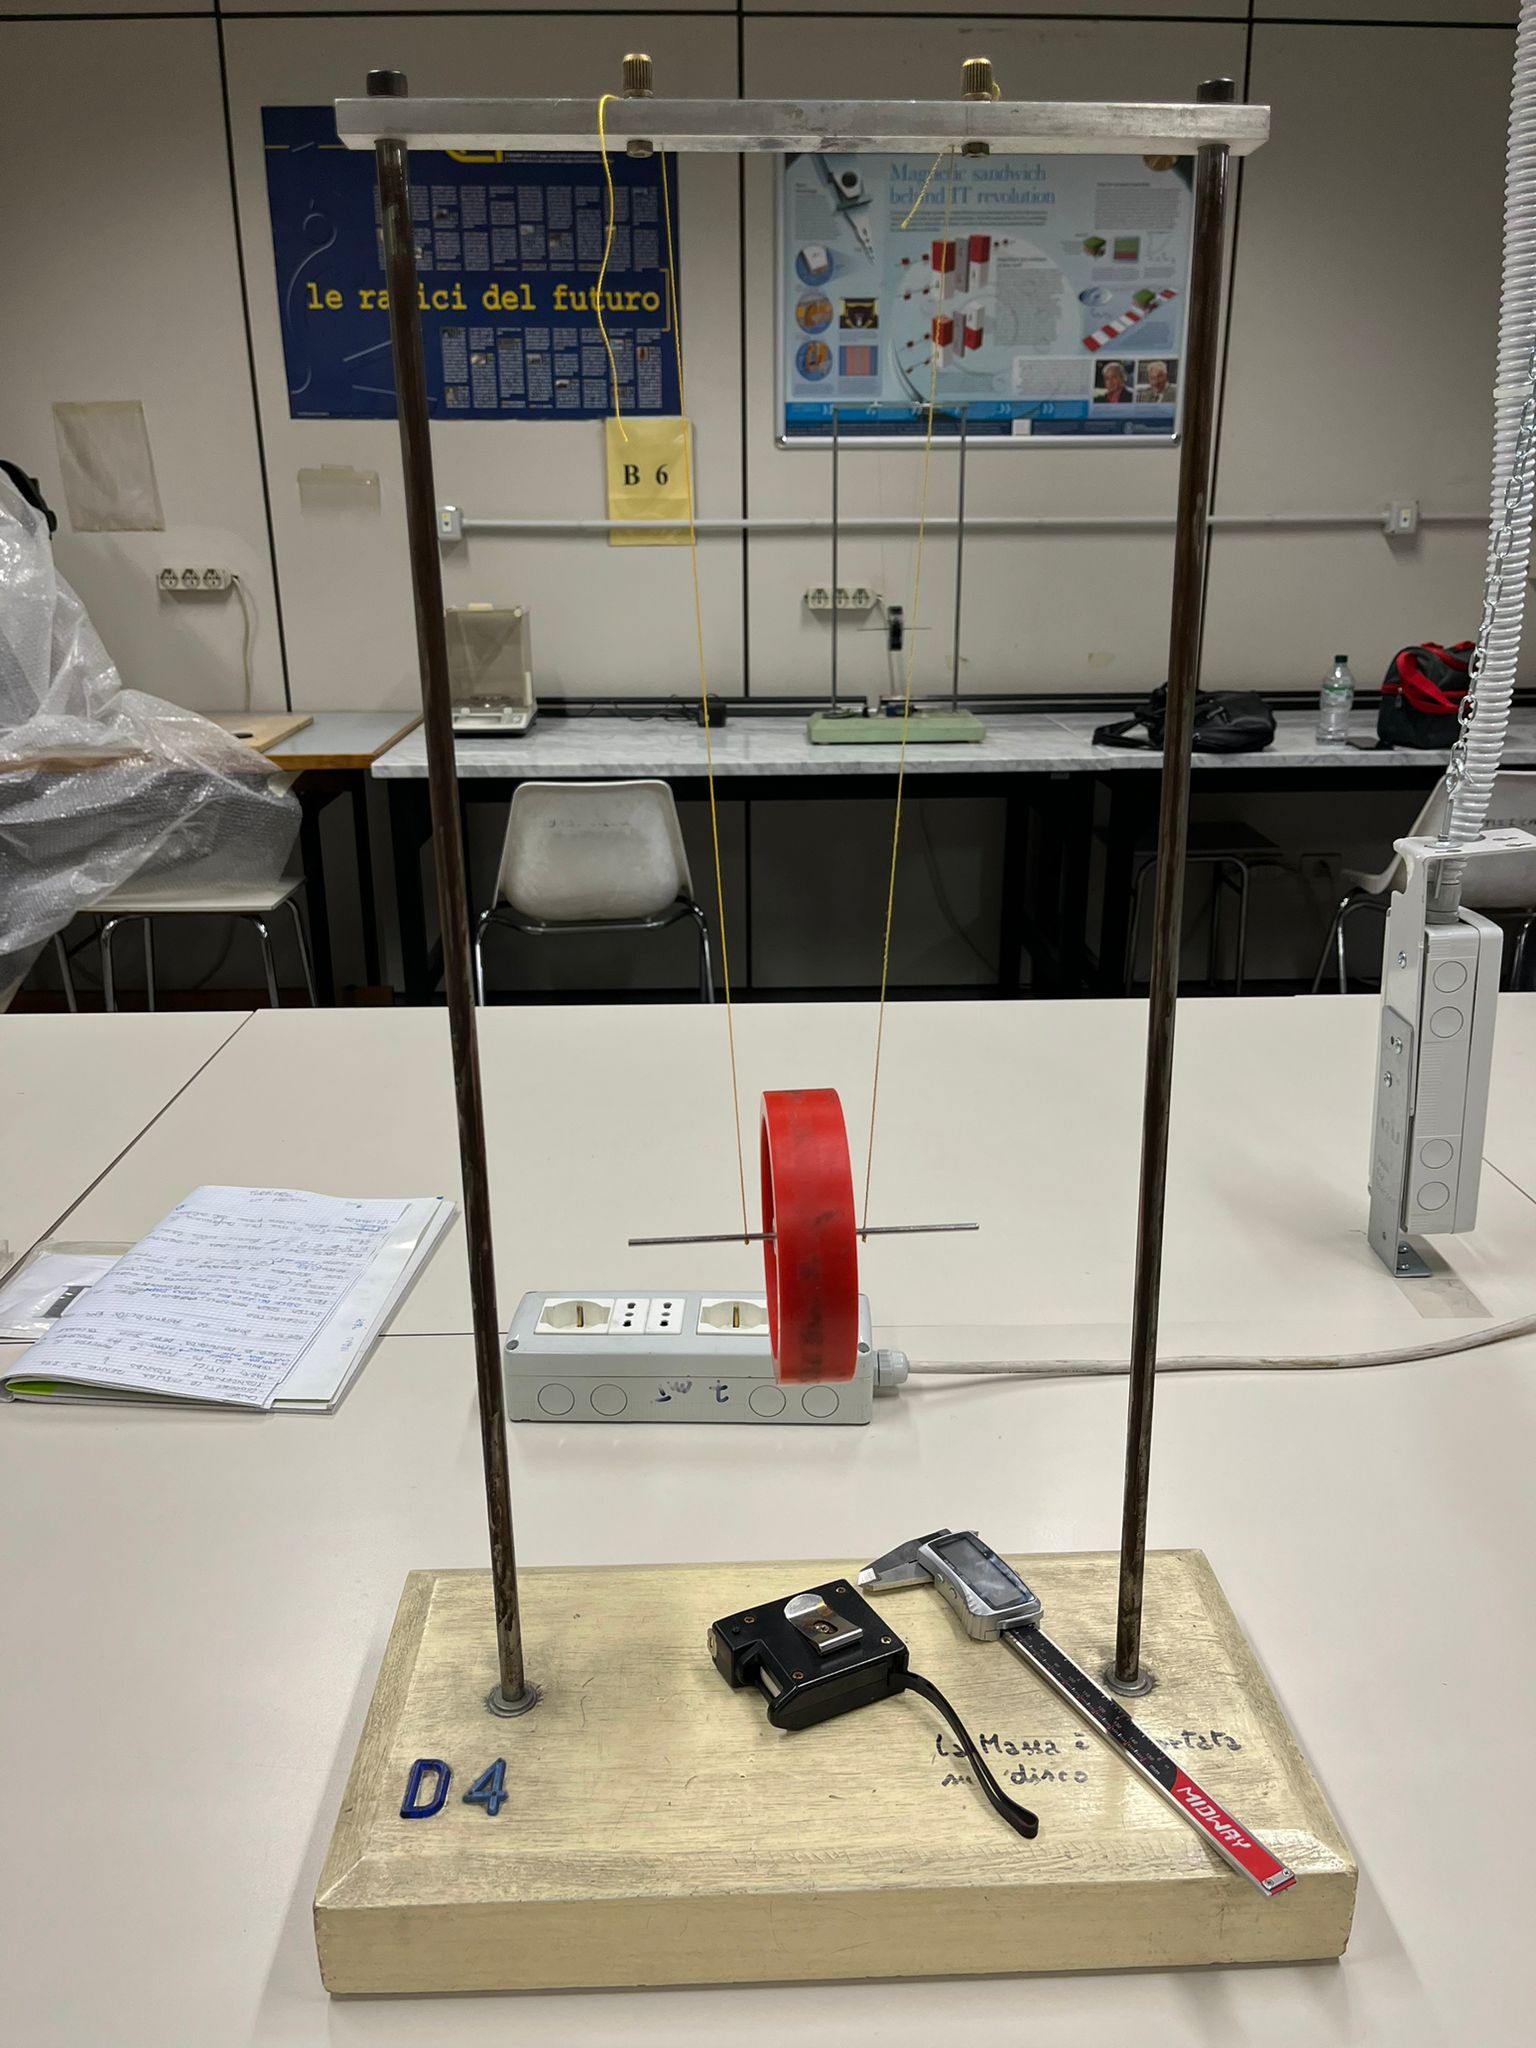
\includegraphics[width=0.4\textwidth]{images/maxwell.jpg}
\caption{Il pendolo di Maxwell utilizzato durante l'esperimento per misurare il momento di inerzia del disco col metodo dinamico.}
\label{maxwell}
\end{figure}

\section{Metodo sperimentale}
\subsection{Apparato sperimentale}
Per misurare i parametri geometrici del pendolo di Maxwell sono stati utilizzati un micrometro, un calibro e un metro, con risoluzioni rispettivamente di $ 1 \cdot 10^{-5} m $, $ 1 \cdot 10^{-5} m $ e $ 1 \cdot 10^{-3} m $. Inoltre, per misurare i tempi di caduta del disco, ci si è serviti del cronometro installato in uno smartphone con risoluzione di $ 1 \cdot 10^{-2} s $. Le fotografie degli strumenti sono riportate nella Fig. \ref{strumenti}.

\begin{figure}[ht!]
\centering
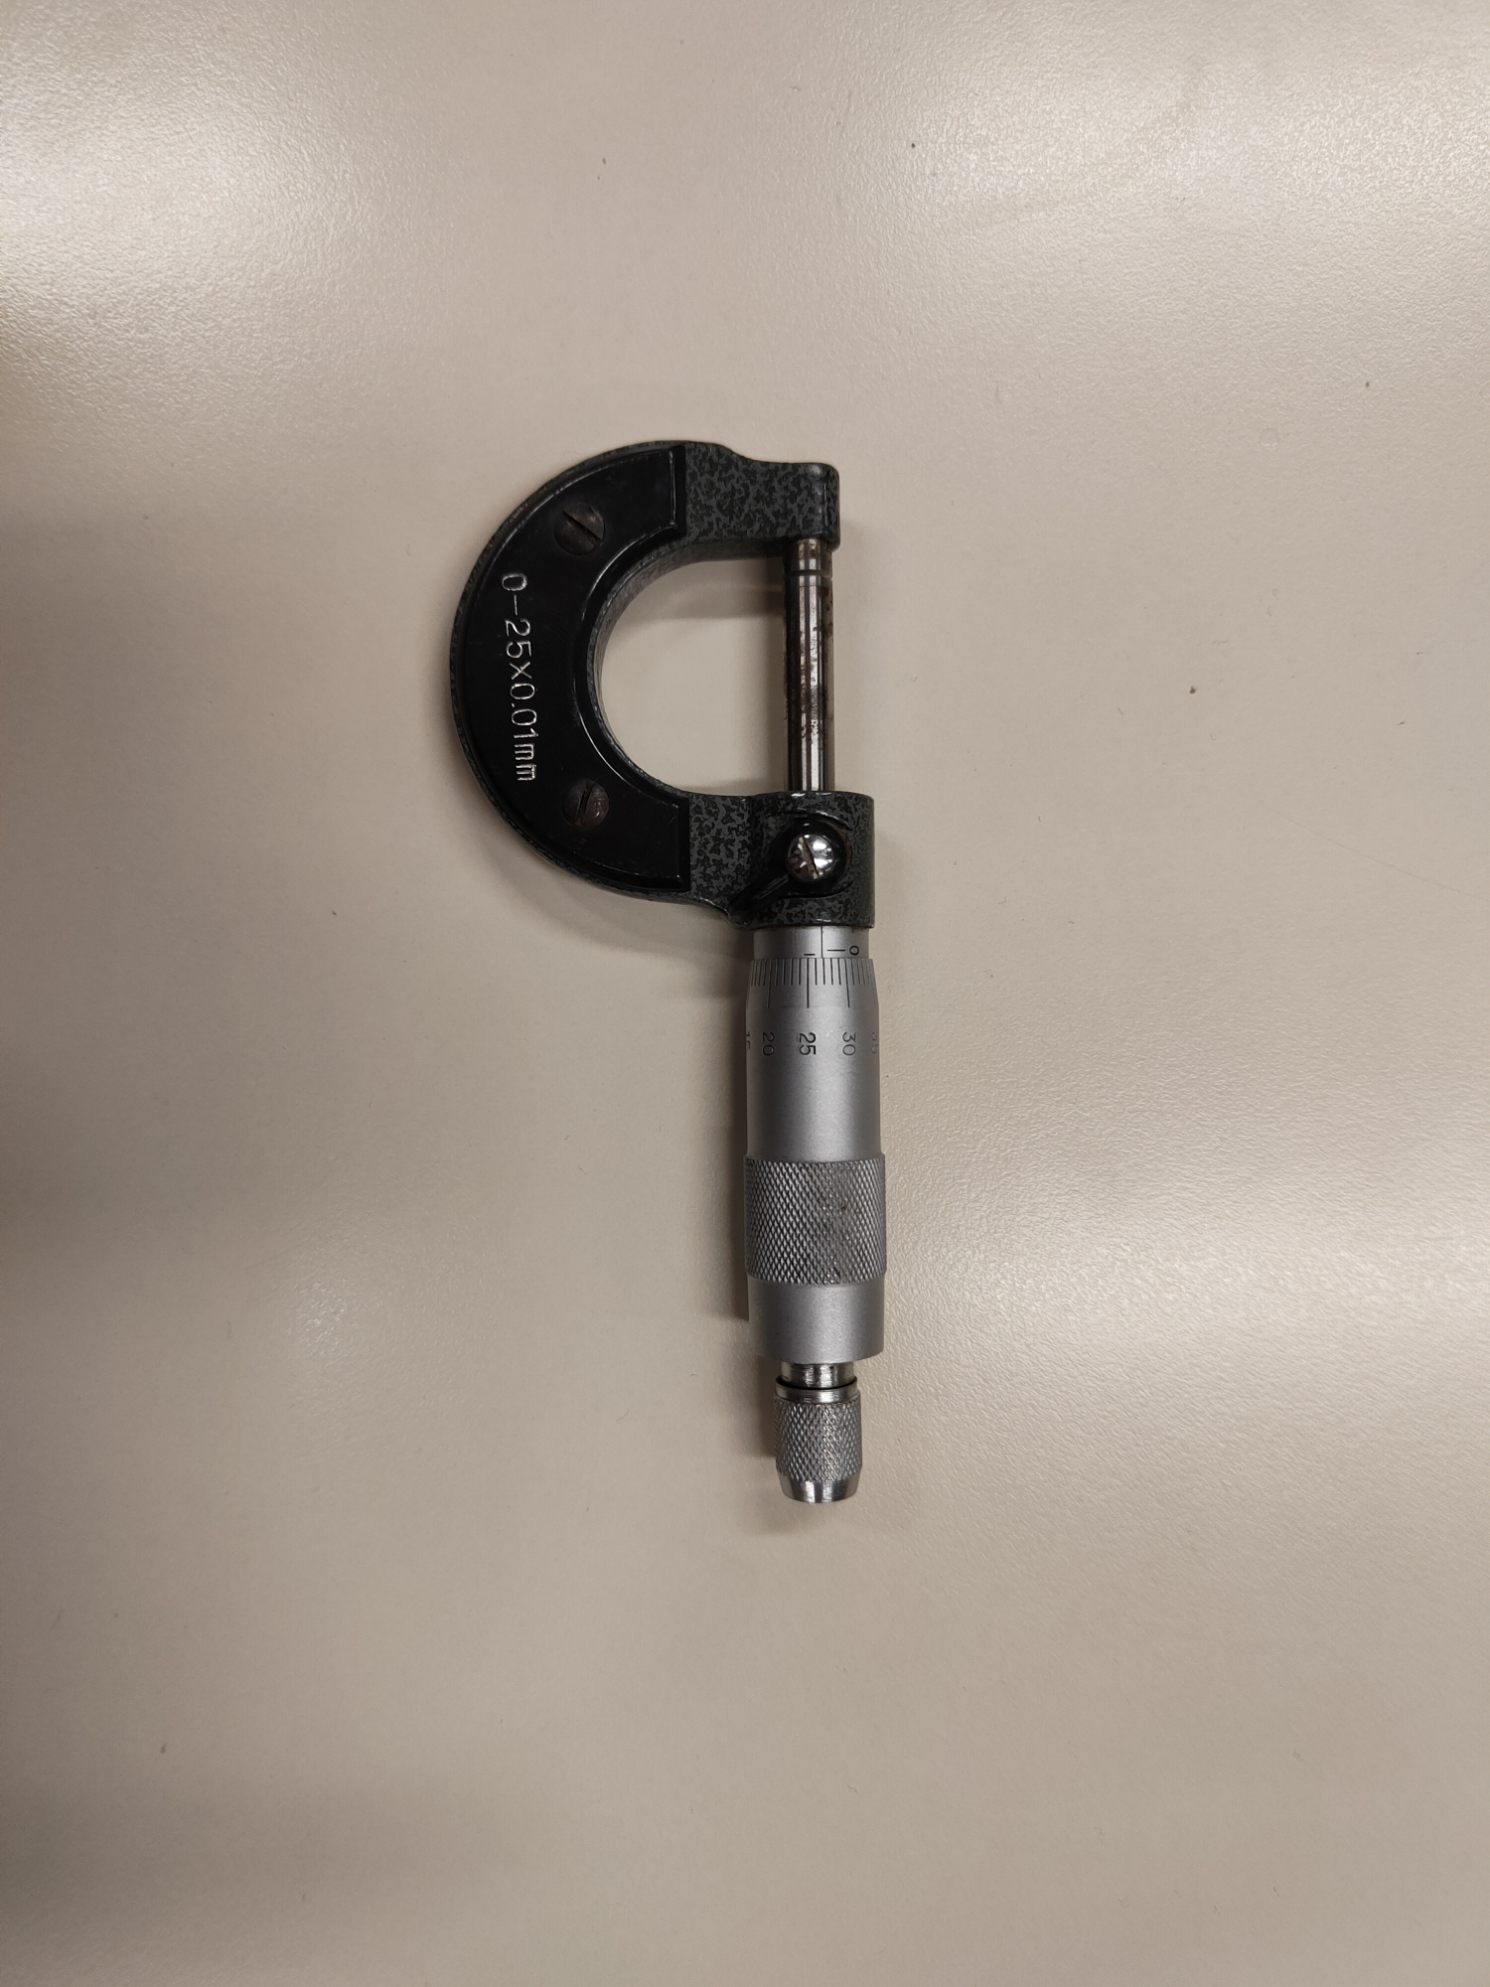
\includegraphics[width=0.23\textwidth]{images/micrometro.jpg}
\hspace{2pt}
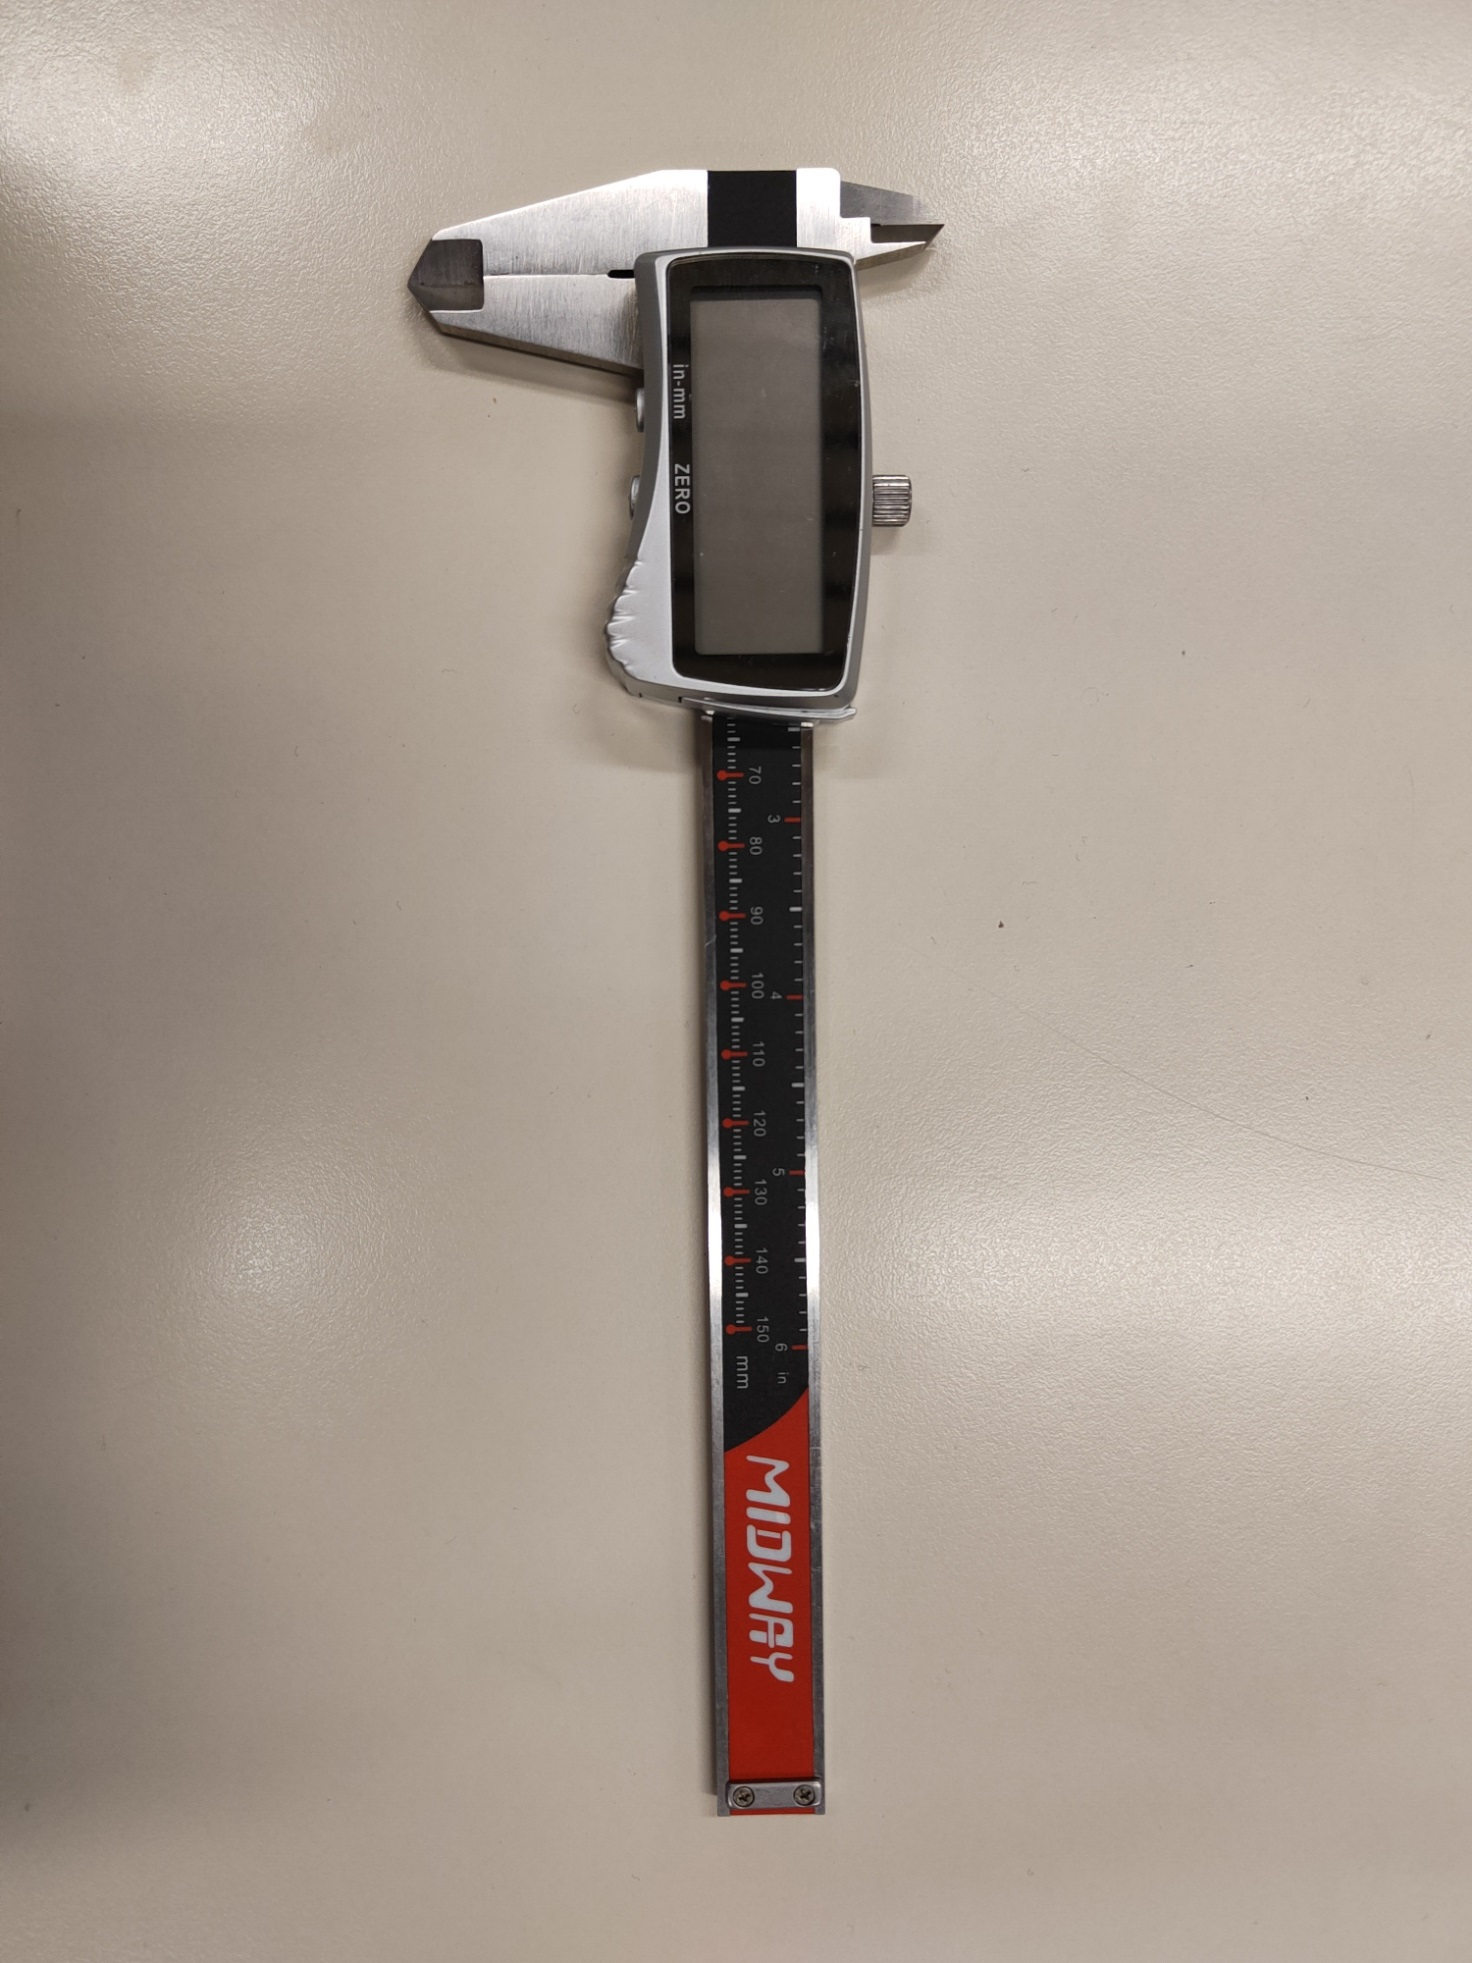
\includegraphics[width=0.23\textwidth]{images/calibro.jpg}
\hspace{2pt}
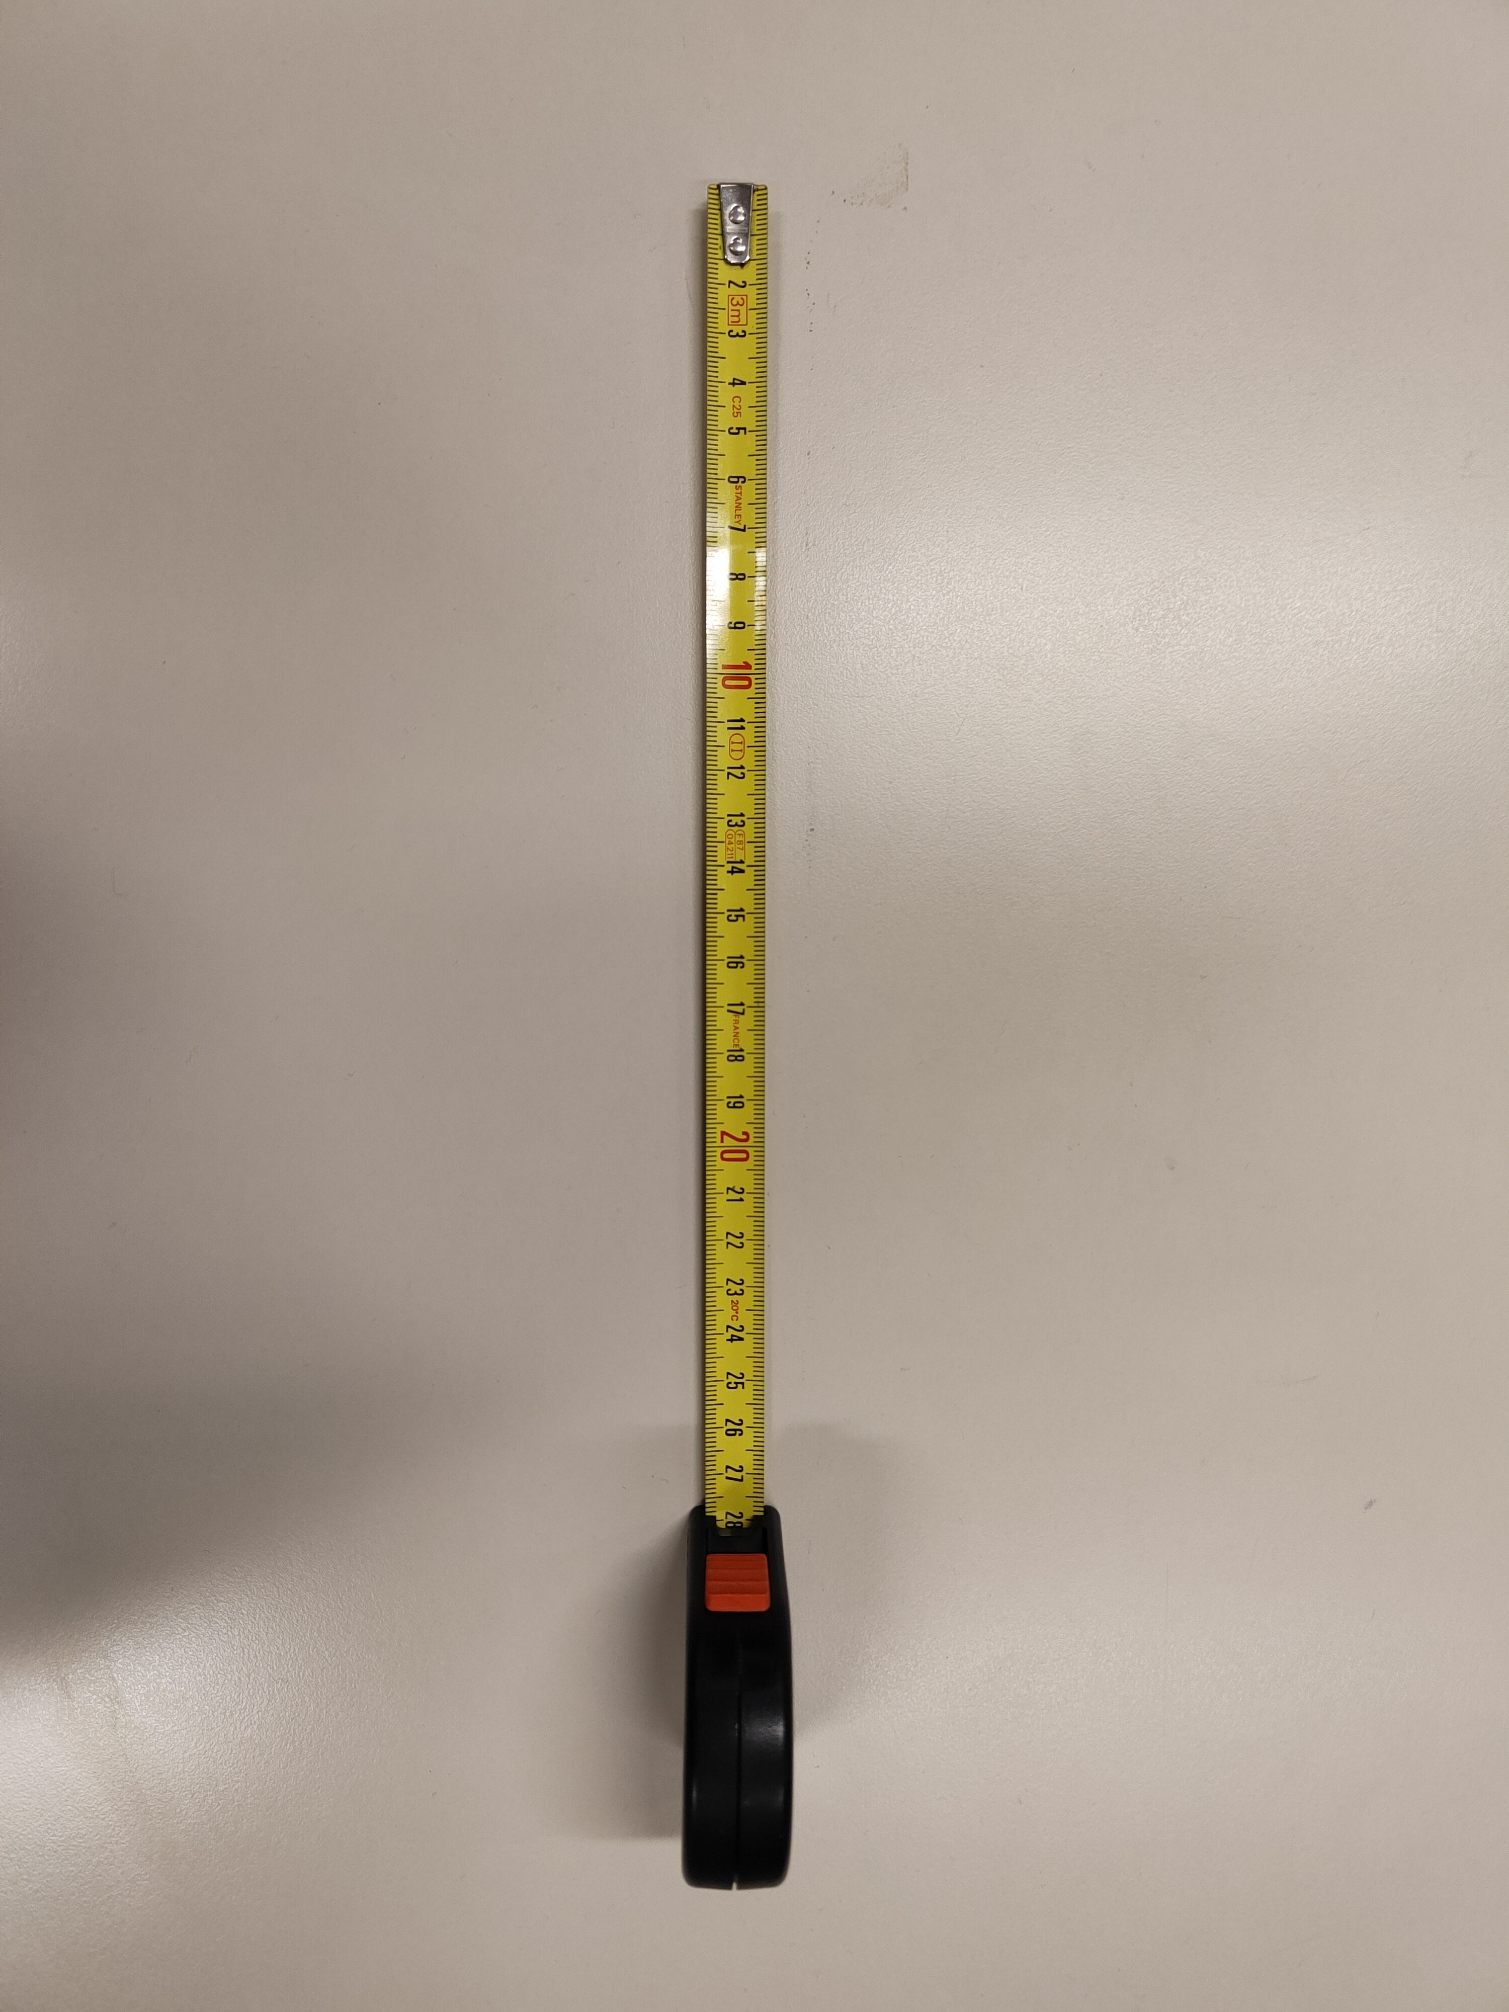
\includegraphics[width=0.23\textwidth]{images/metro.jpg}
\hspace{2pt}
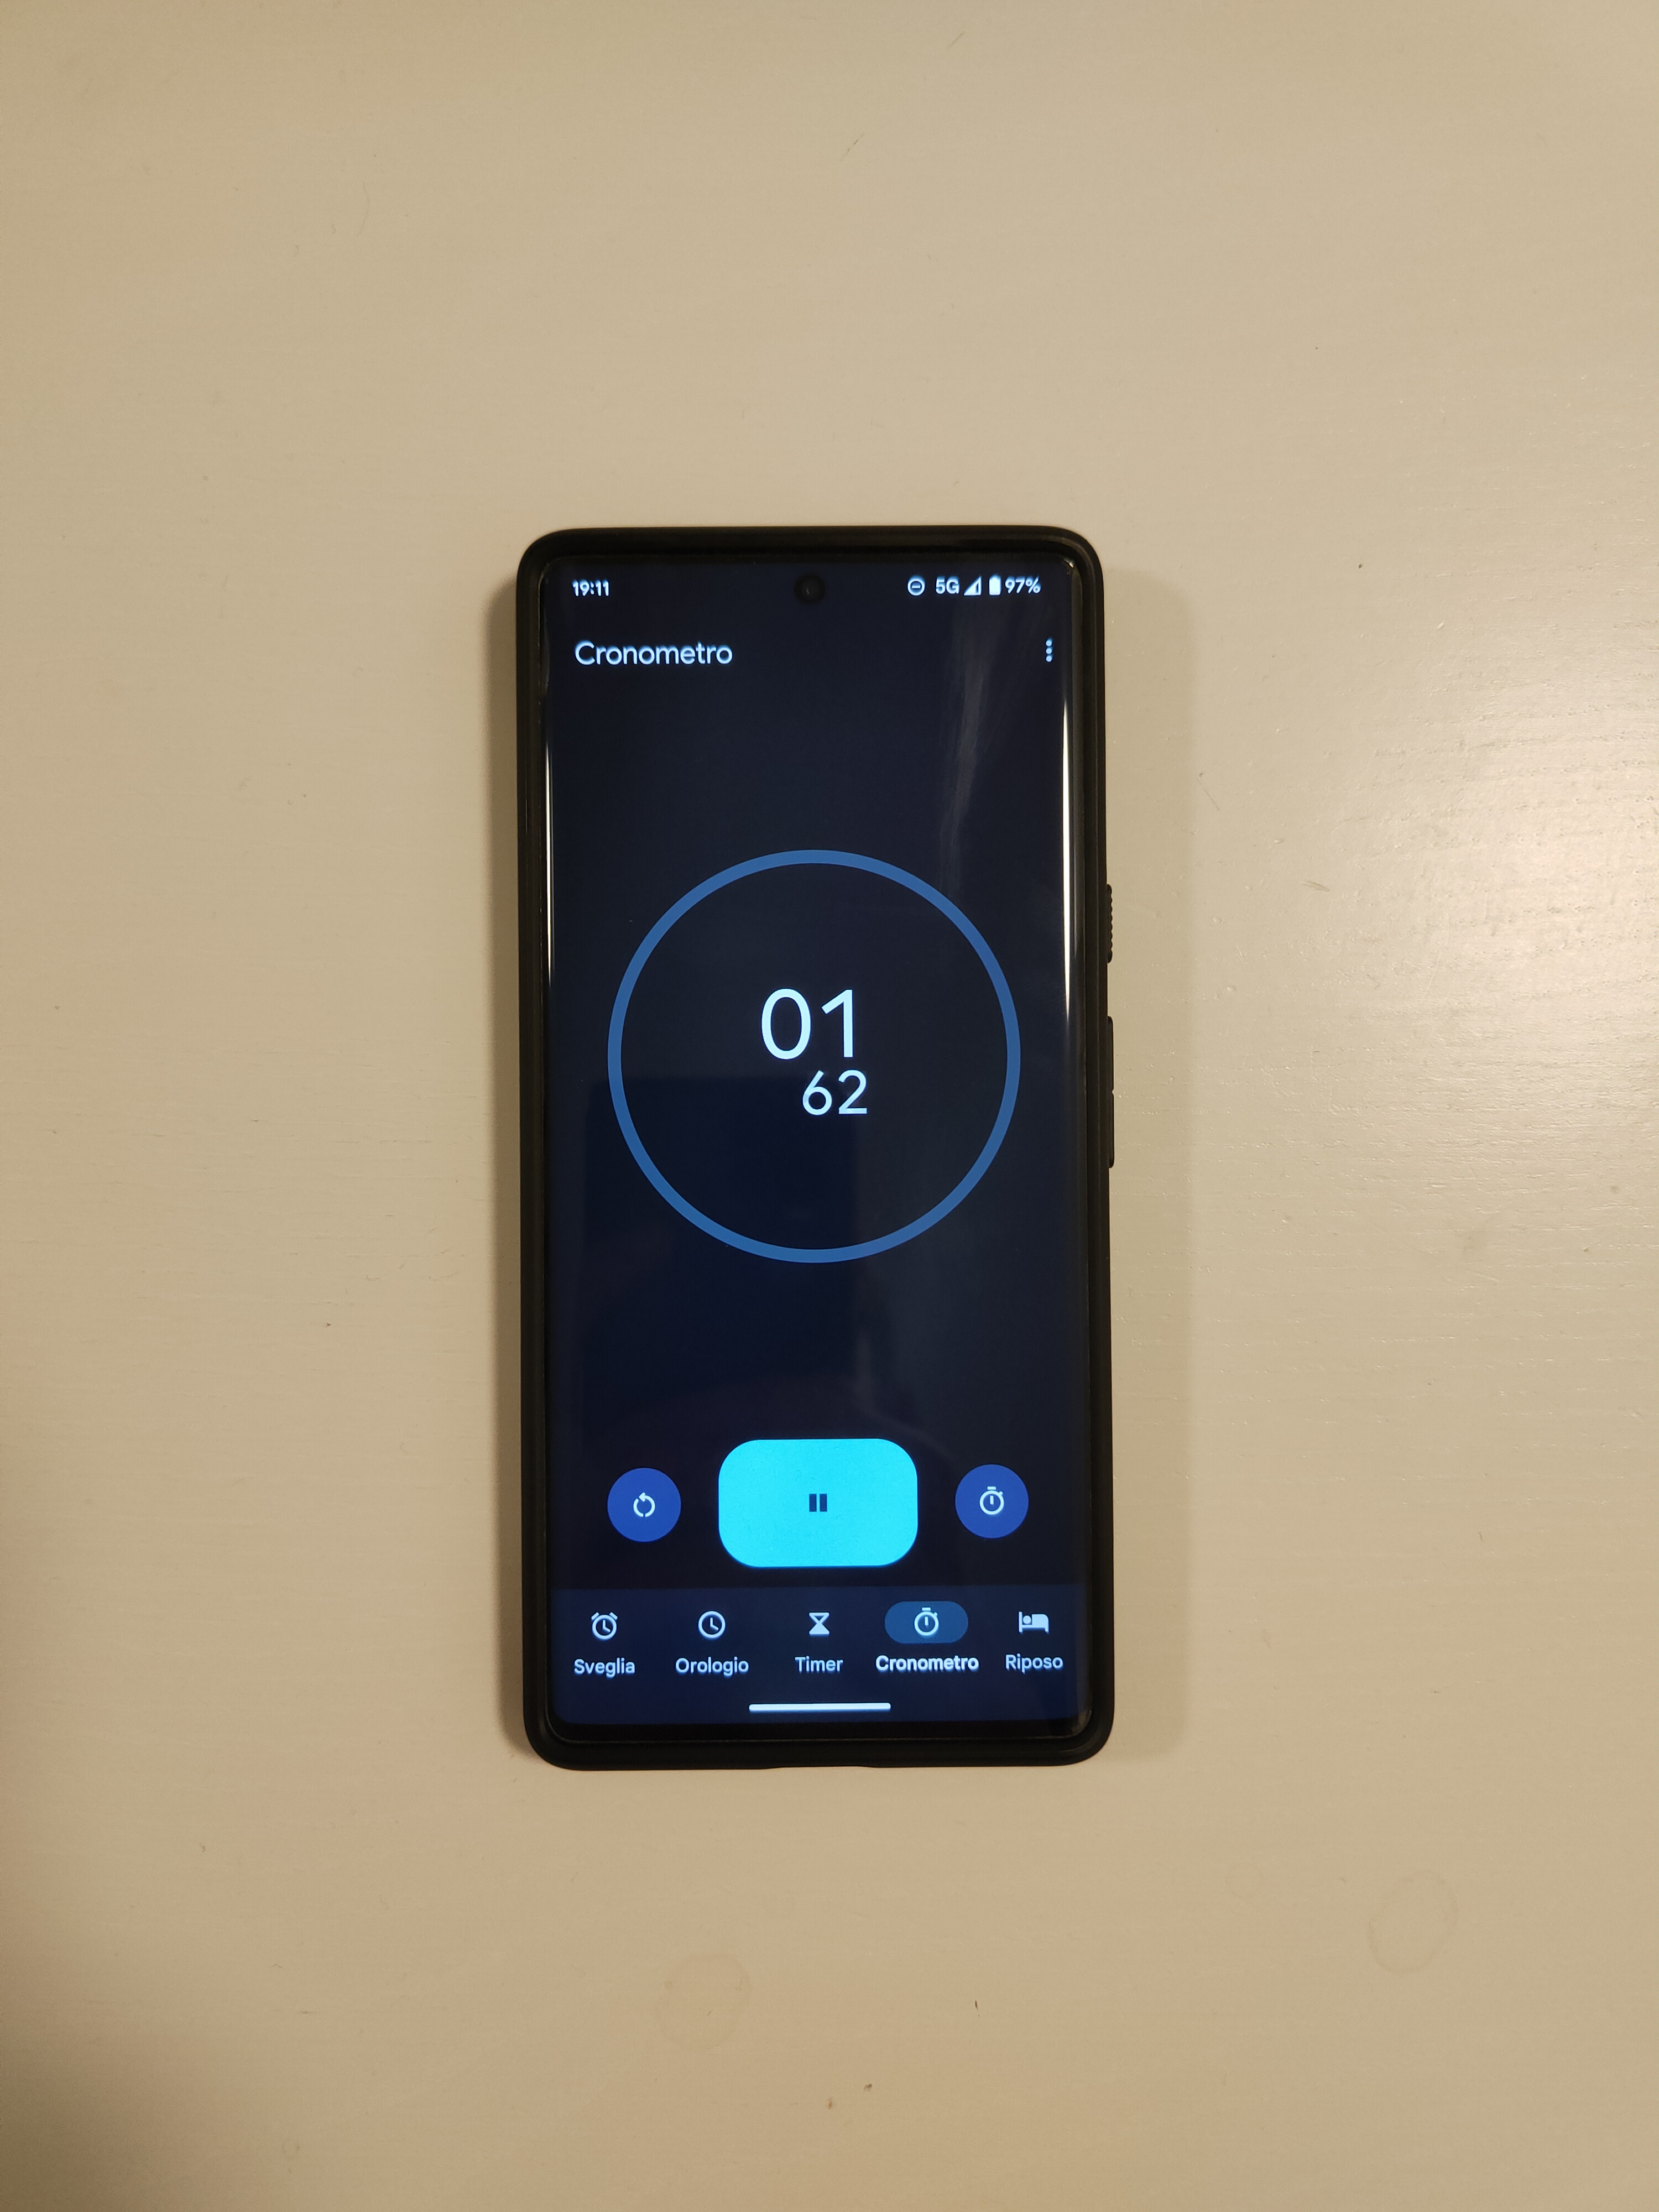
\includegraphics[width=0.23\textwidth]{images/cronometro.jpg}
\caption{Sono riportati in figura, da sinistra a destra, il micrometro, il calibro, il metro e il cronometro utilizzati nel corso dell'esperimento per effettuare le misure dirette.}
\label{strumenti}
\end{figure}

\subsection{Svolgimento}
\subsubsection{Misura dinamica}
\label{svolgimento:dinamica}
Applicando le leggi di conservazione\footnote{Le dissipazioni di energia dovute agli attriti sono state considerate trascurabili.} dell'energia meccanica al disco si può ricavare la seguente espressione per il momento di inerzia\footnote{Per lo svolgimento dei calcoli si veda l'appendice.}:
$$ I = \dfrac{m ( d_{perno} + d_{filo} )^2}{8 h_0} ( g t_0^2 - 2 h_0 ) $$
dove $ m $ è la massa del disco, $ d_{perno} $ il diametro del perno attorno al quale avviene la rotazione, $ d_{filo} $ il diametro dei fili del pendolo di Maxwell, $ h_0 $ e $ t_0 $ rispettivamente l'altezza e il tempo di caduta del disco e $ g $ il modulo dell'accelerazione di gravità in prossimità della crosta terrestre.\\
Dunque, per calcolare il valore di $ I $ è sufficiente conoscere i parametri che compaiono nella sua espressione. A tal fine, sono stati misurati col micrometro $ d_{perno} $ e $ d_{filo} $, mentre $ h_0 $ è stata misurata col metro. I valori $ m = ( 226.0 \pm 0.5 ) g $ e $ g = 9.81 m / s^2 $ erano noti.\\
Successivamente è stato misurato il tempo di caduta per 40 volte, con lo scopo di effettuare un'analisi statistica del campione così ottenuto.
\subsubsection{Misura geometrica}
Il momento di inerzia può essere calcolato anche attraverso la sua definizione: il disco è infatti formato da quattro toroidi a sezione rettangolare omogenei e, dato che si tratta di una grandezza additiva, il momento di inerzia totale è pari alla somma dei momenti di inerzia di ciascun toroide.\\
Il momento di inerzia di un toroide si ricava tramite la formula seguente\footnote{Per la dimostrazione si veda l'appendice.}:
$$ I = \dfrac{\rho \pi z}{2} ( r_{est}^4 - r_{int}^4 ) $$
dove $\rho=(1.36 \pm 0.02)g/cm^3$ è la densità del toroide, $ z $ il suo spessore e $ r_{int} $ e $ r_{est} $ sono, rispettivamente, il suo raggio interno ed esterno.\\
Tutte queste grandezze sono state ricavate servendosi del calibro.

\section{Risultati}

\subsection{Acquisizione dati}
\subsubsection{Misure geometriche}
Le misure relative alla geometria del disco sono riportate nella tabella seguente, in cui $x_{best}$ corrisponde alla media e l'incertezza al valore più alto fra la semidispersione massima e la risoluzione dello strumento. Le misure che iniziano con $d$ indicano un diametro, quelle con $z$ uno spessore e quelle con $h$ un'altezza. Per comprendere a che porzione del disco faccia riferimento ciascuna misura si rimanda allo schema dell'oggetto (Fig. \ref{figure:schema_disco}).

Gli spessori dei quattro toroidi, ad eccezione di $z_4$, sono stati calcolati indirettamente misurando le profondità al bordo del toroide  e sommandole o sottraendole a seconda della situazione allo spessore del toroide adiacente. L'incertezza su questi valori è stata ricavata sommando le incertezze di ciascuno dei termini della somma.

\begin{figure}[ht!]
\centering
\begin{minipage}{.5\textwidth}
\centering
\begin{tabular}{|c|c|}
\hline
 & Valore ($mm$) \\
\hline
$d_{perno}$ & $3.00 \pm 0.01$ \\
\hline
$d_{filo}$ & $2.93 \pm 0.01$ \\
\hline
$h_{0}$ & $333 \pm 1$ \\
\hline
$d_{1}$ & $8.44 \pm 0.02$ \\
\hline
$d_{2}$ & $15.94 \pm 0.01$ \\
\hline
$d_{3}$ & $57.98 \pm 0.01$ \\
\hline
$d_{4}$ & $99.95 \pm 0.05$ \\
\hline
$d_{5}$ & $120.05 \pm 0.02$ \\
\hline
$z_{1}$ & $25.4 \pm 0.3$ \\
\hline
$z_{2}$ & $9.8 \pm 0.2$ \\
\hline
$z_{3}$ & $3.8 \pm 0.1$ \\
\hline
$z_{4}$ & $29.97 \pm 0.02$ \\
\hline
\end{tabular}
\end{minipage}%
\begin{minipage}{.5\textwidth}
\centering
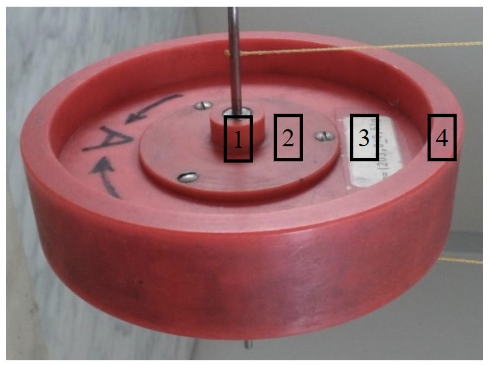
\includegraphics[width=\textwidth]{images/toroide.png}
\end{minipage}
\caption{Il disco è composto da quattro toroidi diversi fra loro. La misura $d_1$ si riferisce al diametro della porzione di perno infilata nel disco, la $d_2$ al diametro esterno del primo toroide rosso e così via. Allo stesso modo, $z_1$ indica lo spessore del primo toroide rosso, $z_2$ quello del secondo e così via.}
\label{figure:schema_disco}
\end{figure}

\subsubsection{Misure dei tempi di caduta del disco}
I tempi di caduta sono stati misurati con il cronometro di un telefono cellulare. Per verificare l'assenza di errori sistematici, il cellulare utilizzato è stato confrontato con un altro sulla misura di un intervallo di tempo di $1000s$. La differenza fra i due strumenti è risultata essere dell'ordine di $10^{-4}s$ ogni $10s$, un divario sufficientemente basso da essere considerato trascurabile. Per tenere conto del possibile errore umano nella presa delle misure, i valori sono stati arrotondati al decimo di secondo. I dati sono stati analizzati prima statisticamente, calcolando i valori sotto riportati per la media ($\overline{x}$), la deviazione standard del campione ($\sigma_{x}$), la deviazione standard della media ($\sigma_{\overline{x}}$) e l'incertezza da associare alla media ($3\sigma_{\overline{x}}$).

\begin{center}
\begin{tabular}{|c|c|c|c|}
\hline
$\overline{x}$ & $\sigma_{x}$ & $\sigma_{\overline{x}}$ & $3\sigma_{\overline{x}}$ \\
\hline
$7.15s$ & $0.1485s$ & $0.0235s$ & $0.0704s$ \\
\hline
\end{tabular}
\end{center}

A partire da questi dati è stata effettuata anche un'analisi grafica con Excel e con il programma di analisi in ROOT, i cui risultati sono riportati nelle figure \ref{figure:tempi_excel} e \ref{figure:tempi_root}. Per ciascun bin è stato calcolato l'integrale della gaussiana cumulativa da $-\infty$ al valore del bin e, sottraendo da ciascuna gaussiana cumulativa la precedente, la probabilità che una misura risulti nel bin in questione. Moltiplicando quest'ultimo risultato per il numero totale di misure effettuate sono stati calcolati gli eventi attesi per ciascun bin. La somma di tutte le frequenze attese è risultata di poco inferiore a 1, così come la somma di tutti gli eventi previsti poco meno di 40, poichè nei bins non compaiono le \quotes{code} della gaussiana.
La figura \quotes{schiacciata} dell'istogramma degli eventi attesi è dovuta al fatto che la media si trova esattamente a metà fra due bins.

\begin{figure}[h!]
\centering
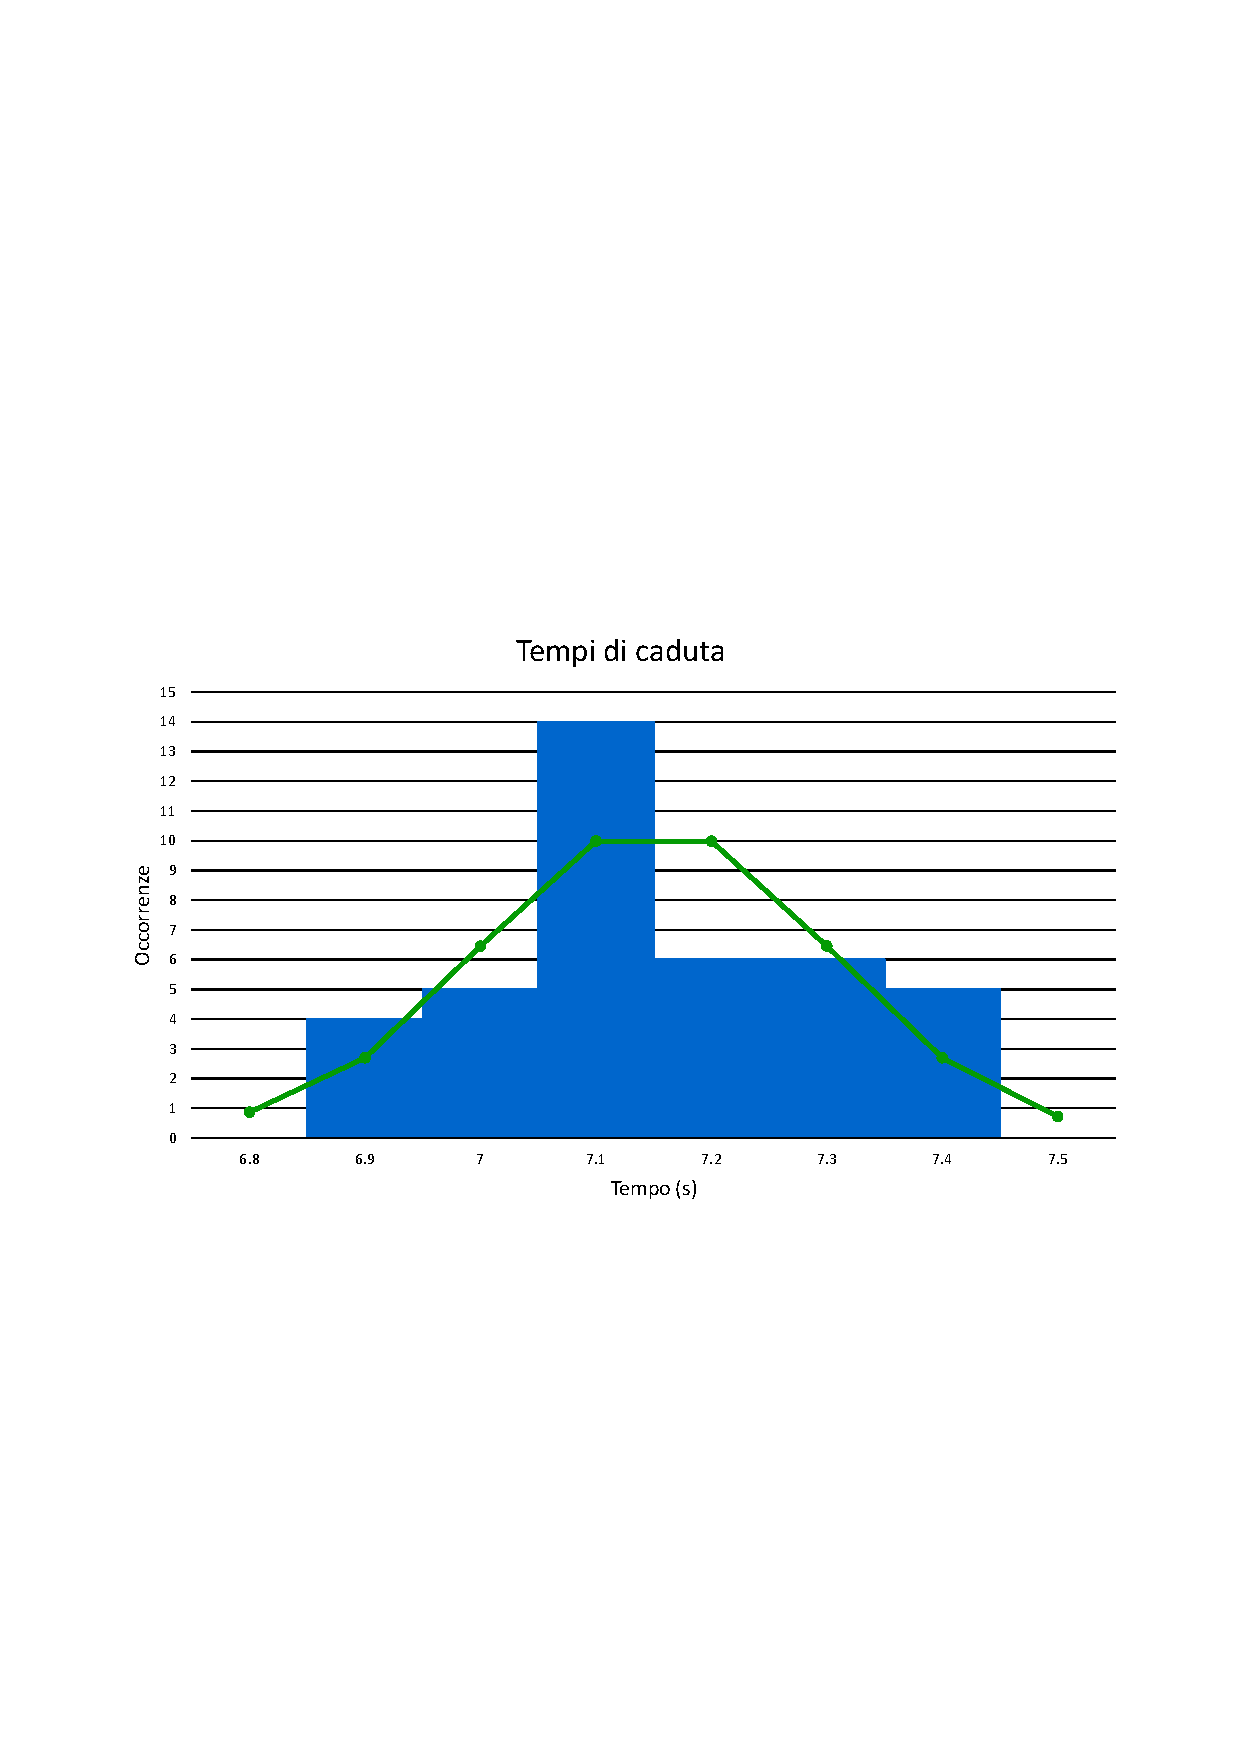
\includegraphics[width=0.7\textwidth]{images/excel.pdf}
\caption{Le colonne blu mostrano le occorrenze dei vari bins. I punti verdi collegati dalla linea rappresentano gli eventi attesi per ciascun bin secondo la distribuzione gaussiana.}
\label{figure:tempi_excel}
\end{figure}

\begin{figure}[h!]
\centering
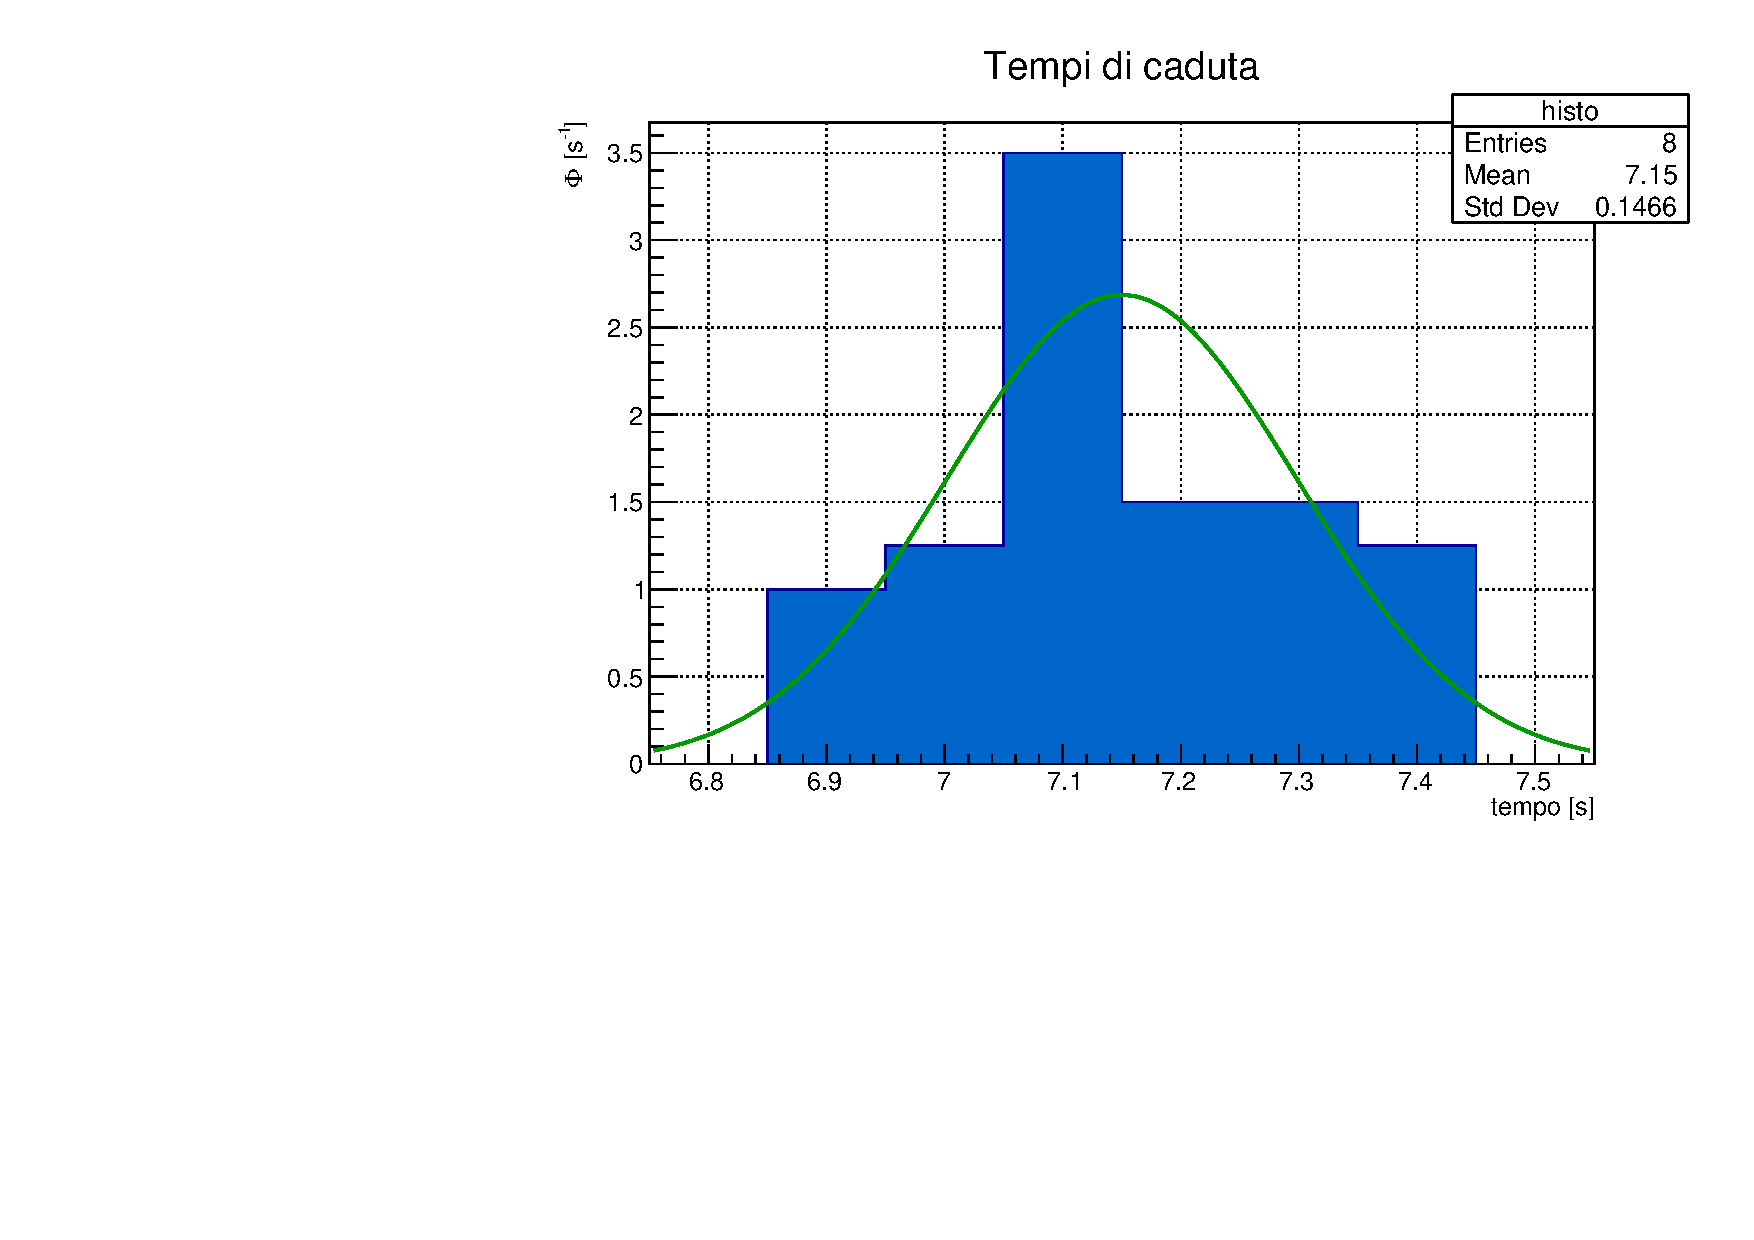
\includegraphics[width=0.7\textwidth]{images/root.pdf}
\caption{Le colonne in blu rappresentano lo stesso istogramma della figura \ref{figure:tempi_excel}, ma in densità di frequenza per poterlo confrontare con la gaussiana generata da ROOT (in verde). \textbf{N.B:} Qui la deviazione standard ha un valore diverso da quella calcolata con Excel e riportata nella tabella precedente. ROOT la calcola infatti utilizzando $N$ al posto di $N-1$ nella definizione.}
\label{figure:tempi_root}
\end{figure}

\subsubsection{Test del $\boldsymbol{\chi ^2}$}
Per verificare l'ipotesi che le misure fossero distribuite normalmente secondo la funzione gaussiana trovata è stato effettuato un test del chi-quadro. Utilizzando la definizione con le misurazioni effettuate si è ottenuto	 il seguente risultato:

$$ \chi ^2 = \displaystyle\sum_{k=1}^8\frac{(O_k-E_k)^2}{E_k} \approx 7.77 $$

\noindent dove $O_k$ sono le occorrenze del $k$-esimo bin e $E_k$ gli eventi attesi nello stesso secondo la distribuzione gaussiana.

In seguito è stato calcolato il chi-quadro ridotto

$$ \widetilde{\chi} ^ 2_0 = \frac{\chi ^ 2}{\nu} \approx 1.55 $$

\noindent dove $ \nu = n - c $ è il numero di gradi di libertà, con $n$ dati osservati e $c$ vincoli. \\
Considerando $8$ dati osservati (il numero dei bins) e $3$ vincoli (il numero totale delle occorrenze, la media e la deviazione standard), si è voluta calcolare la probabilità che, assumendo vera l'ipotesi, si potesse trovare un $\widetilde{\chi} ^ 2 \geq \widetilde{\chi}^2_0$ con $5$ gradi di libertà. Con l'aiuto di una tabella di probabilità del chi-quadro \cite{taylor:chiquadro}, questa probabilità è risultata essere $P_{\nu}(\widetilde{\chi}^2 \geq \widetilde{\chi} ^ 2_0) \approx 17.5 \% \geq 5 \%$, quindi l'ipotesi è stata considerata plausibile.


\subsection{Elaborazione dati e risultati quantitativi}
\subsubsection{Misura dinamica}
Grazie alla legge di conservazione dell'energia meccanica e alle misure dei diametri del perno e del filo, dell'altezza di caduta e dei tempi di caduta è stato possibile calcolare, con l'aiuto di un foglio di calcolo, il momento d'inerzia del disco in maniera dinamica come spiegato precedentemente nella sezione \ref{svolgimento:dinamica}. La sua incertezza relativa è stata trovata con la formula delle incertezze per i prodotti e i quozienti\footnote{Per maggiori dettagli sull'incertezza per prodotti e quozienti si rimanda all'appendice.} \cite{taylor:prodotti}.

$$ \frac{\delta I}{I} = \frac{\delta m}{m} + 2\frac{\delta d_p + \delta d_f}{d_p + d_f} + \frac{\delta h_0}{h_0} + 2\frac{\delta t_0}{t_0} $$

Di seguito sono riportati i contributi di ciascun termine all'incertezza totale. Come si può notare, l'incertezza sulle misurazioni dei tempi è quella che più incide sul valore finale.

\begin{center}
\begin{tabular}{|l|c|}
\hline
Incertezza relativa sulla massa & 0.0022124 \\
Incertezza relativa sui diametri & 0.0121457 \\
Incertezza relativa sull'altezza & 0.0030075 \\
Incertezza relativa sul tempo & 0.0197030 \\
\hline
Incertezza relativa totale & 0.0370686 \\
\hline
\end{tabular}
\end{center}

L'incertezza assoluta sulla misura totale è così risultata essere $0.2 \cdot 10^{-4}kgm^2$. Con la formula per il momento d'inerzia dinamico, trattata sempre nella sezione \ref{svolgimento:dinamica}, è stato calcolato il valore $I_{best}=4.6 \cdot 10^{-4}kgm^2$. Di conseguenza, il valore del momento d'inerzia misurato in maniera dinamica corrisponde a $(4.6 \pm 0.2) \cdot 10^{-4}kgm^2$.

\subsubsection{Misura geometrica}
Poiché il momento d'inerzia è una grandezza additiva, è stato possibile calcolare i contributi dei quattro toroidi separatamente col fine di confrontare la loro influenza sul risultato finale. L'errore sistematico dovuto al non aver considerato il contributo del perno metallico è trascurabile, dato che il momento d'inerzia è direttamente proporzionale al quadrato della distanza dall'asse di rotazione e il perno ha una distanza dall'asse molto piccola rispetto ai toroidi rossi.

\begin{center}
\begin{tabular}{|c|c|c|c|}
\hline
$I_1 (10^{-4}kgm^2)$ & $I_2 (10^{-4}kgm^2)$ & $I_3 (10^{-4}kgm^2)$ & $I_4 (10^{-4}kgm^2)$ \\
\hline
0.002 & 0.148 & 0.454 & 4.318 \\
\hline
\end{tabular}
\end{center}

Il contributo del primo toroide è molto inferiore rispetto agli altri a causa della piccola distanza che lo separa dall'asse di rotazione. Allo stesso modo, il contributo del quarto toroide è nettamente più grande rispetto agli altri (almeno un ordine di grandezza) a causa dell'elevata distanza che intercorre fra esso e il perno metallico.

Utilizzando il metodo delle derivate parziali\footnote{Per la formula ottenuta con le derivate parziali si rimanda all'appendice.}\cite{taylor:derivate} è possibile calcolare l'incertezza anche sulla misura geometrica, che risulta uguale a $0.1 \cdot 10^{-4}kgm^2$. Il valore del momento d'inerzia misurato in modo geometrico è dunque $(4.9 \pm 0.1) \cdot 10^{-4}kgm^2$.

\section{Conclusioni}
L'analisi statistica e grafica dei tempi di caduta restituisce buoni risultati, poichè gli eventi attesi corrispondono con buona approssimazione a quelli effettivamente registrati secondo il test del $\chi ^2$. Con più misurazioni delle cadute del pendolo di Maxwell ci si sarebbe probabilmente avvicinati maggiormente alla curva gaussiana prevista dal programma di analisi in ROOT.

I valori dinamico, $(4.6 \pm 0.2) \cdot 10^{-4}kgm^2$, e geometrico, $(4.9 \pm 0.1) \cdot 10^{-4}kgm^2$, del momento d'inerzia sono risultati compatibili, dal momento che esiste un valore comune ad entrambi gli intervalli di incertezza: $4.8 \cdot 10^{-4}kgm^2$.

\newpage

\begin{thebibliography}{9}
\bibitem{focardi:inerzia}
S. Focardi, I. Massa, A. Uguzzoni, M. Villa, \quotes{Fisica generale - Meccanica e termodinamica}; Casa Editrice Ambrosiana (2014) pag. 349.

\bibitem{taylor:chiquadro}
J. R. Taylor, \quotes{Introduzione all'analisi degli errori}; Zanichelli (2000) pag. 295.

\bibitem{taylor:prodotti}
J. R. Taylor, \quotes{Introduzione all'analisi degli errori}; Zanichelli (2000) pag. 52.

\bibitem{taylor:derivate}
J. R. Taylor, \quotes{Introduzione all'analisi degli errori}; Zanichelli (2000) pag. 75.
\end{thebibliography}

\section*{Appendice}
\paragraph{Espressione del momento di inerzia per la misura dinamica}
Il disco compie un moto roto-traslatorio, dunque la sua energia cinetica consta di una componente traslazionale $ E_{KT} $ e di una rotazionale $ E_{KR} $. Di conseguenza, l'energia meccanica $ E_M $ del disco è:
$$ E_M = E_K + V = E_{KT} + E_{KR} + V = \dfrac{1}{2} m v^2 + \dfrac{1}{2} I \omega ^2 + m g y = \dfrac{1}{2} m \dot{y}^2 + \dfrac{1}{2} I \dfrac{\dot{y}^2}{r^2} + m g y $$
dove $ r $ è la distanza tra il centro del filo e l'asse di rotazione, quindi $ r = \dfrac{d_{perno} + d_{filo}}{2} $.\\
Dato che l'energia meccanica si conserva, si ha che $ \dot{E}_M = 0 $. Di conseguenza:
$$ m \dot{y} \ddot{y} + \dfrac{I}{r^2} \dot{y} \ddot{y} + m g \dot{y} = 0 \quad \Longleftrightarrow \quad \ddot{y} = - \dfrac{m g}{m + \dfrac{I}{r^2}} $$
Quindi il centro di massa del disco subisce un'accelerazione $ \vv{a} $ rivolta verso il basso di modulo:
$$ \abs{\vv{a}} = \abs{\ddot{y}} = \dfrac{m g}{m + \dfrac{I}{r^2}} $$
Chiamando $ h_0 $ lo spazio percorso durante la caduta e $ t_0 $ il tempo impiegato per cadere, grazie alla legge oraria del moto uniformemente accelerato è possibile ricavare $ I $:
\begin{gather*}
h_0 = \dfrac{1}{2} a t_0^2 = \dfrac{1}{2} \dfrac{m g}{m + \dfrac{I}{r^2}} t_0^2 \quad \Longleftrightarrow \quad \left( m + \dfrac{I}{r^2} \right) h_0 = \dfrac{1}{2} m g t_0^2 \quad \Longleftrightarrow \quad \dfrac{I}{r^2} h_0 = \dfrac{1}{2} m g t_0^2 - m h_0 \quad \Longleftrightarrow \\
\Longleftrightarrow \quad I = \dfrac{m r^2}{2 h_0} ( g t_0^2 - 2 h_0 ) = \dfrac{m \left( \dfrac{d_{perno} + d_{filo}}{2} \right) ^2}{2 h_0} ( g t_0^2 - 2 h_0 ) = \dfrac{m ( d_{perno} + d_{filo} )^2}{8 h_0} ( g t_0^2 - 2 h_0 )
\end{gather*}

\paragraph{Momento di inerzia di un toroide a sezione rettangolare}
Si consideri un toroide a sezione rettangolare di cui sono note densità $ \rho $, raggio interno $ r_{int} $, raggio esterno $ r_{est} $ e altezza $ z $.\\
La definizione del momento di inerzia è:
$$ I = \int_V r ^ 2 dm = \int_V r ^ 2 \rho dV $$
Per trovare $ dV $ si consideri un incremento infinitesimo $ dr $ della distanza dall'asse di rotazione. Dato che $ dr $ è una lunghezza infinitesima, $ dV $ è pari al volume del parallelepipedo di larghezza $ 2 \pi r $, altezza $ z $ e profondità $ dr $:
$$ dV = 2 \pi r z dr $$
Sostituendo nella definizione di $ I $ si ricava la seguente formula:
$$ I = \int_V r ^ 2 \rho dV = \int_{r_{int}}^{r_{est}} r ^ 2 \rho \left( 2 \pi r z dr \right) = 2 \pi \rho z \int_{r_{int}}^{r_{est}} r ^ 3 dr = 2 \rho \pi z \left( \dfrac{r_{est} ^ 4}{4} - \dfrac{r_{int} ^ 4}{4} \right) = \dfrac{\rho \pi z}{2} \left( r_{est} ^ 4 - r_{int} ^ 4 \right) $$


\paragraph{Calcolo dell'incertezza per prodotti e quozienti}
Per grandezze che sono definite come prodotti o quozienti nella cui espressione nessuna variabile compare più di una volta, quindi della forma $q(x,y,\ldots, z) = cx^{\alpha}y^{\beta} \cdots z^{\omega}$ dove $c$ è una costante numerica, l'incertezza relativa è uguale a

$$ \frac{\delta q}{q} = |\alpha|\frac{\delta x}{x} + |\beta|\frac{\delta y}{y} + \cdots + |\omega|\frac{\delta z}{z}  $$

\paragraph{Calcolo dell'incertezza geometrica con le derivate parziali}
Come mostrato precedentemente,

$$ I = \frac{\rho \pi}{32}[z_1(d_2^4-d_1^4)+z_2(d_3^4-d_2^4)+z_3(d_4^4-d_3^4)+z_4(d_5^4-d_4^4)].$$

Essendo questa una funzione in più variabili, è opportuno calcolare l'incertezza sulla quantità $I$ tramite le derivate parziali invece che con il metodo \quotes{passo per passo}. Infatti, in generale, per una funzione di più variabili $q(x,y,\ldots)$ vale

$$ \delta q(x,y,\ldots) = \bigg|\frac{\partial q}{\partial x}\bigg|_{x_{best},y_{best},\ldots}\delta x + \bigg|\frac{\partial q}{\partial y}\bigg|_{x_{best},y_{best},\ldots}\delta y + \cdots $$

Per utilizzare questa formula è necessario calcolare la derivata parziale del momento d'inerzia rispetto a ciascuna variabile.

$$ \bigg|\frac{\partial I}{\partial \rho}\bigg| = \frac{I}{\rho} \thinspace , \qquad \bigg|\frac{\partial I}{\partial z_i}\bigg| = \frac{\rho \pi}{32}|d_{i+1}^4-d_i^4| \thinspace , \qquad \bigg|\frac{\partial I}{\partial d_1}\bigg| = \frac{\rho \pi}{8}z_1d_1^3 \thinspace , \qquad \bigg|\frac{\partial I}{\partial d_{2}}\bigg| = \frac{\rho \pi}{8}|z_{1}-z_{2}|d_{2}^3$$

$$ \bigg|\frac{\partial I}{\partial d_{3}}\bigg| = \frac{\rho \pi}{8}|z_{2}-z_{3}|d_{3}^3 \thinspace , \qquad \bigg|\frac{\partial I}{\partial d_{4}}\bigg| = \frac{\rho \pi}{8}|z_{3}-z_{4}|d_{4}^3 \thinspace , \qquad \bigg|\frac{\partial I}{\partial d_5}\bigg| = \frac{\rho \pi}{8}z_4d_5^3 $$

L'incertezza totale è il risultato della somma di tutte le derivate parziali moltiplicate per le rispettive incertezze.

$$ \delta I = \frac{I}{\rho} \delta \rho + \frac{\rho \pi}{8}[z_1d_1^3 \delta d_1 + |z_1-z_2|d_2^3 \delta d_2 + |z_2-z_3|d_3^3 \delta d_3 + |z_3-z_4|d_4^3 \delta d_4 + z_4d_5^3 \delta d_5] + \displaystyle\sum_{i=1}^{4}\frac{\rho \pi}{32}|d_{i+1}^4-d_i^4| \delta z_i $$

\end{document}
